\section{Methods}
\label{sec:Methods}

\subsection{Model description}
\label{subsec:Model}

We focused our attention on food webs with two trophic levels, one of consumers and another of prey (see figure \ref{fig:Network} in the Online Appendix). The consumers predate on the prey, and the prey populations compete among each other for a common source of resources. 

% Description of the dynamics
The dynamics were modelled as a system of ordinary differential equations. We used the Rosenzweig-MacArthur predator-prey model \cite{Rosenzweig1963} generalized to a higher number of species (see \cite{Scheffer2004} and Online Appendix). 

Our model contains $n_P$ prey species and $n_C$ predator species. The prey's populations grow logistically under the influence of intra and interspecific competition. The intensities of both these competitions are coded in the matrix $A$. The coupling of both groups happens via predation. Obviously, predation has a negative effect for prey and a positive one for predators. The relative preference that predators show to each prey is coded in the matrix $S$. In the absence of prey, the predators' populations just decay exponentially. Prey immigration from neighboring areas has been added to the classical model in order to avoid unrealistic long-stretched cycles with near extinctions \cite{Scheffer2004}.

In mathematical notation, the system reads:

\begin{eqnarray}
\label{eq:SystemUnderStudy}
	\begin{cases} 
	P_i'(t) =  r_i(P) P_i  - P_i \sum_{j = 1}^{n_C} g_j(P) S_{ji} C_j + f & : i = 1..n_P
	\\
	C_j'(t) = - l C_j +  e g_j(P) C_j \sum_{i = 1}^{n_P} S_{ji} P_i & : j = 1..n_C
	\end{cases}
\end{eqnarray}

where $P_i(t)$ represents the biomass of prey species $i$ at time $t$ and $C_j(t)$ the biomass of predator species $j$ at time $t$. The auxiliary functions $r_i(P)$ and $g_j(P)$ have been respectively chosen to generalize the logistic growth and the Holling type II saturation functional response \cite{Edelstein-Keshet} to a multispecies system when inserted into equation \ref{eq:SystemUnderStudy}. They are defined as:

\begin{eqnarray}
\label{eq:HollingGenerator}
	r_i(P) = r \left( 1 - \frac{1}{K} \sum_{k=1}^{n_P} A_{ik} P_k \right)
	\\
	g_j(P) = \frac{g}{\sum_{i=1}^{n_P} S_{ji} P_i + H}
\end{eqnarray}

For details about the parameters used, please refer to subsection \ref{subsec:Parameterization}. For a detailed derivation of equation \ref{eq:SystemUnderStudy}, see Online Appendix.

\subsection{Parameterization}
\label{subsec:Parameterization}
We parameterized our model as a freshwater plankton system based on Dakos' model \cite{Dakos2009b}. Dakos' model uses a Rosenzweig-McArthur multi-species model with two trophic levels, and parameterizes it to describe a zooplankton - phytoplankton system. Unlike Dakos, who uses seasonally changing parameters, our parameters were assumed to be independent of time (see table \ref{tab:Parameters}).

\begin{table}[H]
	\begin{center}
		\resizebox{\columnwidth}{!}{
		\begin{tabular}{|c|c|c|c|}
			\hline
			\textbf{Symbol} & \textbf{Interpretation} & \textbf{Value} & \textbf{Units} \\
			\hline
			$r$ & Maximum growth rate & $0.50$ & $d^{-1}$ \\
		    \hline
			$K$ & Carrying capacity & $10.00$ & $ mg \ l^{-1} $ \\
			\hline
			$g$ & Predation rate & $0.40$ & $d^{-1}$\\
			\hline
			$f$ & Immigration rate & $10^{-5}$ & $mg \ l^{-1} \ d^{-1}$\\
			\hline
			$e$ & Assimilation efficiency & $0.60$ & $1$\\
			\hline
			$H$ & Half-saturation constant & $2.00$ & $ mg \ l^{-1} $\\
		    \hline
			$l$ & Predator's loss rate & $0.15$ & $d^{-1}$\\
			\hline
		    $S$ & $ n_C \times n_P $ predator preference matrix & $S_{ij} \in (0,1)$ & $1$\\
		    \hline
   		    $A$ & $ n_P \times n_P $ competition matrix & See section \ref{subsubsec:CompetitionParameter} & $1$\\
		    \hline
		\end{tabular}}
	\end{center}
	\caption{Values and meanings of the parameters used in our numerical experiment. The elements of the predation matrix $S$ are drawn from a uniform probability distribution, bounded between $0$ and $1$.}
	\label{tab:Parameters}
\end{table}

\subsubsection{Competition matrix}
\label{subsubsec:CompetitionParameter}

Our main purpose is to analyze the effect of different degrees of heterogeneity in the competition matrix on the long term dynamics exhibited. In order to simulate and quantify this heterogeneity, we introduce the competition parameter $ \epsilon $. This dimensionless parameter was used to build a competition matrix $A$, whose diagonal terms are identically $ 1 $, and whose non-diagonal terms are drawn from a uniform probability distribution centered at $ 1 + \epsilon $ and with a given width (here we chose $ w = 0.2$).

Defined this way, the parameter $\epsilon$ allows us to travel continuously from strong intraspecific ($ \epsilon < 0$) to strong interspecific competition ($ \epsilon > 0$), meeting neutral competition near $\epsilon = 0$ (see figure \ref{fig:CompetitionParameter}).

\begin{figure}[H]
	\begin{center}
		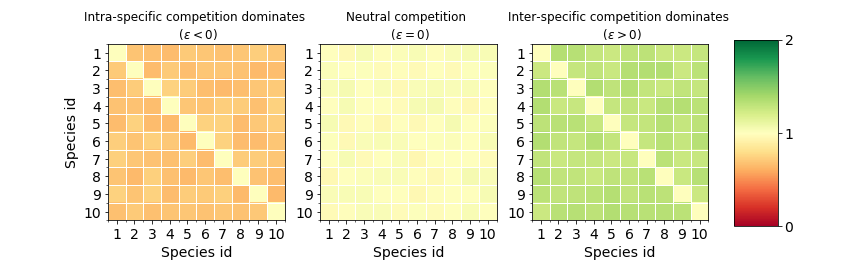
\includegraphics[width=1\columnwidth]{epsilon_all.png}
	\end{center}
	\caption{The competition matrix on the left is a clear case of dominant intraspecific competition. The central one represents a case of neutral competition. The matrix in the right panel shows a case of dominant interspecific competition. The difference between them is the relative size of the non-diagonal elements respective of the diagonal ones. This qualitative property of the competition matrices is controlled by the competition parameter $\epsilon$.}	
	\label{fig:CompetitionParameter}
\end{figure}

\subsection{Numerical experiment}
\label{subsec:NumericalExperiment}

Depending on the parameters and initial conditions, a system like the one described in equation \ref{eq:SystemUnderStudy} can give rise to three types of qualitative behaviour. Each of them roughly corresponds to a different type of attractor (see figure \ref{fig:TimeSeries}). The first one, a stable point attractor, generates a constant species composition. Secondly, limit cycle (and limit tori) attractors give rise to periodically (or quasiperiodically) changing species composition. Lastly, we'll refer as chaotic to attractors that, while remaining bounded, do not fit in any of the previous categories.

\begin{figure}
	\begin{center}
		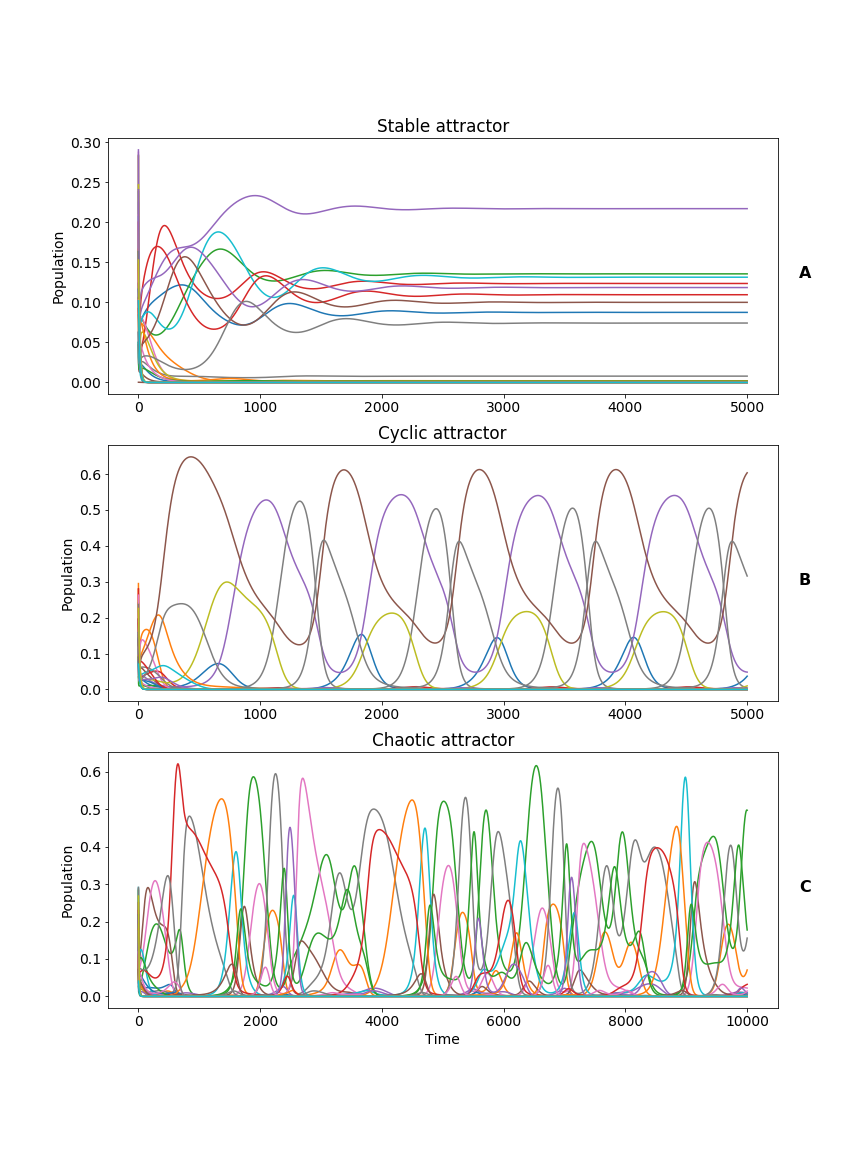
\includegraphics[width=1\columnwidth]{ts.png}
	\end{center}
	\caption{Our family of models generates time series of the population of each species. The time series can be classified in $3$ qualitative types depending on their asymptotic behaviour: \textit{stable}, \textit{periodic} and \textit{chaotic}. In \textbf{panel A}, the system reaches a stable attractor after a transient time. In \textbf{panel B}, a periodic attractor, with an approximate period of 1000 days, is reached after the transient time. The system in \textbf{panel C} never reaches a stable nor a cyclic attractor, but a chaotic one.}
	\label{fig:TimeSeries}
\end{figure}

Our target is to estimate the probability of reaching one of such chaotic attractors under different assumptions about competition. In order to achieve this, we swept among $\numEpsilons$ different values of the competition parameter $\epsilon$ (defined in section \ref{subsubsec:CompetitionParameter}). We simulated a set of $\numReps$ ecosystems per competition parameter value. This amounts to a total of $\numExps$ simulated ecosystems. These ecosystems differ from each other in initial conditions, predation rates $S_{ji}$, and competition matrices, all of them sampled from probability distributions (see \ref{subsec:Parameterization}). Ecosystems grouped by competition parameter $\epsilon$, despite not being identical, exhibit the same competition type (see \ref{subsubsec:CompetitionParameter}).

Numerical methods were used to integrate each realization of the equation \ref{eq:SystemUnderStudy}. A first stabilizing run of $ \stabilTime $ days is executed in order to get closer to the attractor. Simulating for $ \simTime $ more days, we obtain trajectories in the vicinity of the attractor.

We considered chaotic those time series that triggered the Gottwald - Melbourne test (see\cite{Gottwald2009} and Online Appendix). Using this approach, we classified each individual simulation as \textit{chaotic} or \textit{non-chaotic}.

The ratio of attractors found to be chaotic can be used to estimate the probability of a family of ecosystems to develop chaotic behaviour. Grouping those ecosystems by competition parameter $\epsilon$, we explored the relationship between the probability of chaos and the degree of heterogeneity.

Additionally, the experiment was repeated for food webs of different sizes. In our simulations, we kept a ratio of 2:3 for the number of species at the consumer and the prey level.

For the sake of reproducibility, we provide a \textit{GitHub} link to the analysis scripts used\footnote{\url{https://github.com/PabRod/Chaos-and-neutrality}}.